\section{Elongated bodies}

\begin{itemize}
  \item Here we look at the second oblique branch of the $St_L-\AR$ plane. Here we have already found that for $\AR=5$ the first mode to become unstable is mode QS, i.e. the quasi-subharmonic mode.
  \item We now investigate what happens when increasing $\AR$. We recall that this is the range where the vortex shedding is dominated by the TE. This means that the dynamics of the TE vortex shedding dominates and is not directly influenced by the vortex shedding from the LE as in the oblique branches. As shown in figure \ref{fig:mult_AR5s}, for $\AR=5$ the only unstable mode is of subharmonic nature and is the so-called mode $QS$. As $\AR$ is increased, instead, a new mode of synchronous nature appears (in this case the multipliers are real and positive). For $\AR=5.25$ this mode is stable. For $\AR=5.35$ this mode approaches the unit circle. For $\AR=5.5$ this mode is unstable, and its growth rate is larger than the corresponding one associated with mode $QS$. The second mode here detected resembles mode $A$ for the wake past short cylinders. 
  \item Mode QS is an unstable mode of the recirculating region along the lateral sides of the cylinder. This is visualised in figure \ref{fig:mult_AR5s} (note that the mote is maximum there and not in the wake). For additional details see \citep{chiarini-etal-2022}. The synchronous mode, instead, is an unsteady mode of the wake and share several properties with the classical mode $A$ of the circular cylinder.
  \item For the arise of the new mode $A$ in the $5.25 \le \AR \le 5.75$ regime look at the works by Aleksyuk \& Heil (2023) and Aleksyuk \& Heil (2024). To answer the question "Why this mode is not detected for $\AR=5$? Why it becomes unstable only at larger $\AR$?" We can start looking whether also in this case the mechanism proposed by Aleksyuk \& Heil (2023,2024) works. If this is the case, we can see if for $\AR=5$ we actually have something different. 
  \item \textcolor{blue}{For $\AR=5.5$ we have that mode $A'$ and $QS$ become unstable is short succession. We can use DNS to see how do they appear. We start from $Re=450$ and then increase progressively $Re$. Look for an indicator to characterise how the flow moves from one regime to the other.}
\end{itemize}

%For the arise of the new mode $A$ in the $5.25 \le \AR \le 5.75$ regime look at the works by Aleksyuk \& Heil (2023) and Aleksyuk \& Heil (2024)


\begin{figure}
  \centering
%  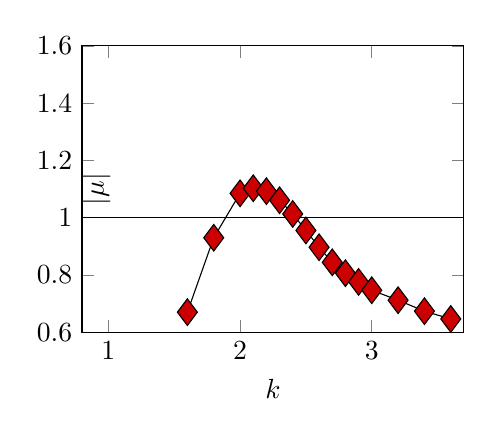
\begin{tikzpicture}



\begin{axis}[%
%width=4.3cm,
%height=3.5cm,
width=0.4\textwidth,
height=0.3\textwidth,
%width=0.2\textwidth,
%height=0.2\textwidth,
scale only axis,
%grid=both,
%axis lines=middle,
xmin=0.8,
xmax=3.7,
ymin=0.6,
ymax=1.6,
%xtick={2, 3, 4, 5, 6, 7, 8, 9, 10, 11},
%ytick={2, 2.5, 3, 3.5, 4, 4.5, 5, 5.5, 6, 6.5, 7},
%xlabel style={font=\color{white!15!black}},
xlabel={$k$},
ylabel={$|\mu|$},
ylabel style={at={(0.1,0.5)}},
%ymin=0,
%ymax=200,
axis background/.style={fill=white},
legend style={at={(0.99,0.85)}, anchor=east, legend cell align=left, align=left, fill=none, draw=none}
]


\addplot [color=black,solid,mark=diamond*,mark options={scale=2.4,black,fill=red!80!black}]
  table[row sep=crcr]{%
   %1.000000000000000   1.000070000000000 \\
  % 1.300000000000000   0.714343000000000 \\
   1.600000000000000   0.670046000000000 \\
   1.800000000000000   0.929885000000000 \\
   2.000000000000000   1.085060000000000 \\
   2.100000000000000   1.102700000000000 \\
   2.200000000000000   1.092560000000000 \\
   2.300000000000000   1.060710000000000 \\
   2.400000000000000   1.012990000000000 \\
   2.500000000000000   0.955412000000000 \\
   2.600000000000000   0.896718000000000 \\
   2.700000000000000   0.844065000000000 \\
   2.800000000000000   0.806200000000000 \\ 
   2.900000000000000   0.775755000000000 \\ 
   3.000000000000000   0.746579000000000 \\
   3.200000000000000   0.711819000000000 \\
   3.400000000000000   0.673520000000000 \\
   3.600000000000000   0.646376000000000 \\
   %4.000000000000000   0.562545000000000 \\
   %4.800000000000000   0.530527000000000 \\
   %5.000000000000000   0.524629000000000 \\
   %5.400000000000000   0.489231000000000 \\
   %5.800000000000000   0.468024000000000 \\
   %6.200000000000000   0.448075000000000 \\
};
%\addlegendentry{$Re=500$}

\addplot [color=black,solid,mark=,mark options={scale=1.4,black,fill=green!80!black}]
  table[row sep=crcr]{%
  0 1 \\
  5 1 \\
};





\end{axis}

\end{tikzpicture}%

%  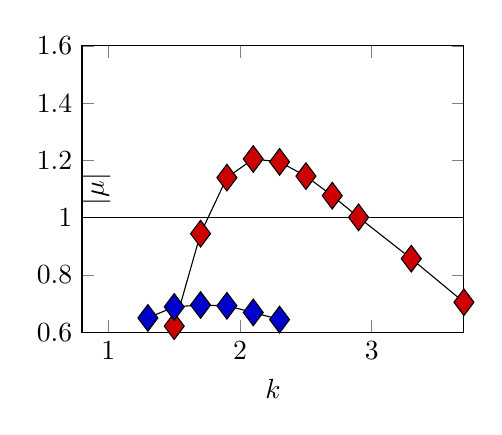
\begin{tikzpicture}



\begin{axis}[%
%width=4.3cm,
%height=3.5cm,
width=0.4\textwidth,
height=0.3\textwidth,
%width=0.2\textwidth,
%height=0.2\textwidth,
scale only axis,
%grid=both,
%axis lines=middle,
xmin=0.8,
xmax=3.7,
ymin=0.6,
ymax=1.6,
%xtick={2, 3, 4, 5, 6, 7, 8, 9, 10, 11},
%ytick={2, 2.5, 3, 3.5, 4, 4.5, 5, 5.5, 6, 6.5, 7},
%xlabel style={font=\color{white!15!black}},
xlabel={$k$},
ylabel={$|\mu|$},
ylabel style={at={(0.1,0.5)}},
%ymin=0,
%ymax=200,
axis background/.style={fill=white},
legend style={at={(0.99,0.85)}, anchor=east, legend cell align=left, align=left, fill=none, draw=none}
]


\addplot [color=black,solid,mark=diamond*,mark options={scale=2.4,black,fill=red!80!black}]
  table[row sep=crcr]{%
1.5 0.621431 \\
1.7 0.944234 \\
1.9 1.13979 \\
2.1 1.20487 \\
2.3 1.19477 \\
2.5 1.14503 \\
2.7 1.07689 \\
2.9 1.00122 \\
3.3 0.856827 \\
3.7 0.704753 \\
};
\addplot [color=black,solid,mark=diamond*,mark options={scale=2.4,black,fill=blue!80!black}]
  table[row sep=crcr]{%
1.3 0.650088 \\
1.5 0.688449 \\
1.7 0.695007 \\
1.9 0.692386 \\
2.1 0.669215 \\
2.3 0.644222 \\
};


%\addlegendentry{$Re=500$}

\addplot [color=black,solid,mark=,mark options={scale=2.4,black,fill=green!80!black}]
  table[row sep=crcr]{%
  0 1 \\
  5 1 \\
};





\end{axis}

\end{tikzpicture}%

%  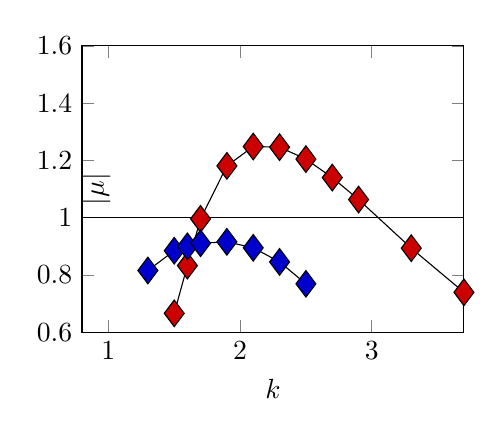
\begin{tikzpicture}



\begin{axis}[%
%width=4.3cm,
%height=3.5cm,
width=0.4\textwidth,
height=0.3\textwidth,
%width=0.2\textwidth,
%height=0.2\textwidth,
scale only axis,
%grid=both,
%axis lines=middle,
xmin=0.8,
xmax=3.7,
ymin=0.6,
ymax=1.6,
%xtick={2, 3, 4, 5, 6, 7, 8, 9, 10, 11},
%ytick={2, 2.5, 3, 3.5, 4, 4.5, 5, 5.5, 6, 6.5, 7},
%xlabel style={font=\color{white!15!black}},
xlabel={$k$},
ylabel={$|\mu|$},
ylabel style={at={(0.1,0.5)}},
%ymin=0,
%ymax=200,
axis background/.style={fill=white},
legend style={at={(0.99,0.85)}, anchor=east, legend cell align=left, align=left, fill=none, draw=none}
]


\addplot [color=black,solid,mark=diamond*,mark options={scale=2.4,black,fill=red!80!black}]
  table[row sep=crcr]{%
1.5 0.666004 \\
1.6 0.832646 \\
1.7 0.9958 \\
1.9 1.18082 \\
2.1 1.24832 \\
2.3 1.24618 \\
2.5 1.20433 \\
2.7 1.14004 \\
2.9 1.06321 \\
3.3 0.893504 \\
3.7 0.739385 \\
};
\addplot [color=black,solid,mark=diamond*,mark options={scale=2.4,black,fill=blue!80!black}]
  table[row sep=crcr]{%
1.3 0.815608 \\
1.5 0.884647 \\
1.6 0.899934 \\
1.7 0.910632 \\
1.9 0.915668 \\
2.1 0.89476 \\
2.3 0.845626 \\
2.5 0.769004 \\
%2.7 0.733247 \\
};


%\addlegendentry{$Re=500$}

\addplot [color=black,solid,mark=,mark options={scale=1.4,black,fill=green!80!black}]
  table[row sep=crcr]{%
  0 1 \\
  5 1 \\
};





\end{axis}

\end{tikzpicture}%
  
%  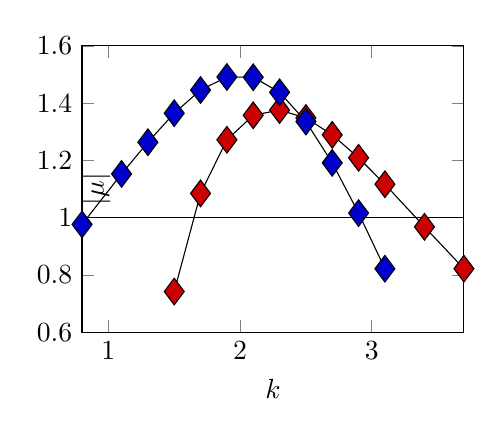
\begin{tikzpicture}



\begin{axis}[%
%width=4.3cm,
%height=3.5cm,
width=0.4\textwidth,
height=0.3\textwidth,
%width=0.2\textwidth,
%height=0.2\textwidth,
scale only axis,
%grid=both,
%axis lines=middle,
xmin=0.8,
xmax=3.7,
ymin=0.6,
ymax=1.6,
%xtick={2, 3, 4, 5, 6, 7, 8, 9, 10, 11},
%ytick={2, 2.5, 3, 3.5, 4, 4.5, 5, 5.5, 6, 6.5, 7},
%xlabel style={font=\color{white!15!black}},
xlabel={$k$},
ylabel={$|\mu|$},
ylabel style={at={(0.1,0.5)}},
%ymin=0,
%ymax=200,
axis background/.style={fill=white},
legend style={at={(0.99,0.85)}, anchor=east, legend cell align=left, align=left, fill=none, draw=none}
]


\addplot [color=black,solid,mark=diamond*,mark options={scale=2.4,black,fill=red!80!black}]
  table[row sep=crcr]{%
1.5 0.742066 \\
1.7 1.08482 \\
1.9 1.27188 \\
2.1 1.35744 \\
2.3 1.3757 \\
2.5 1.34816 \\
2.7 1.28908 \\
2.9 1.20902 \\
3.1 1.11666 \\
3.4 0.968 \\
3.7 0.821928 \\
};
\addplot [color=black,solid,mark=diamond*,mark options={scale=2.4,black,fill=blue!80!black}]
  table[row sep=crcr]{%
0.8 0.976452 \\
1.1 1.1528 \\
1.3 1.26332 \\
1.5 1.36481 \\
1.7 1.44557 \\
1.9 1.49116 \\
2.1 1.49023 \\
2.3 1.43771 \\
2.5 1.33553 \\
2.7 1.1913 \\
2.9 1.01607 \\
3.1 0.821755 \\
};


%\addlegendentry{$Re=500$}

\addplot [color=black,solid,mark=,mark options={scale=1.4,black,fill=green!80!black}]
  table[row sep=crcr]{%
  0 1 \\
  5 1 \\
};





\end{axis}

\end{tikzpicture}%

  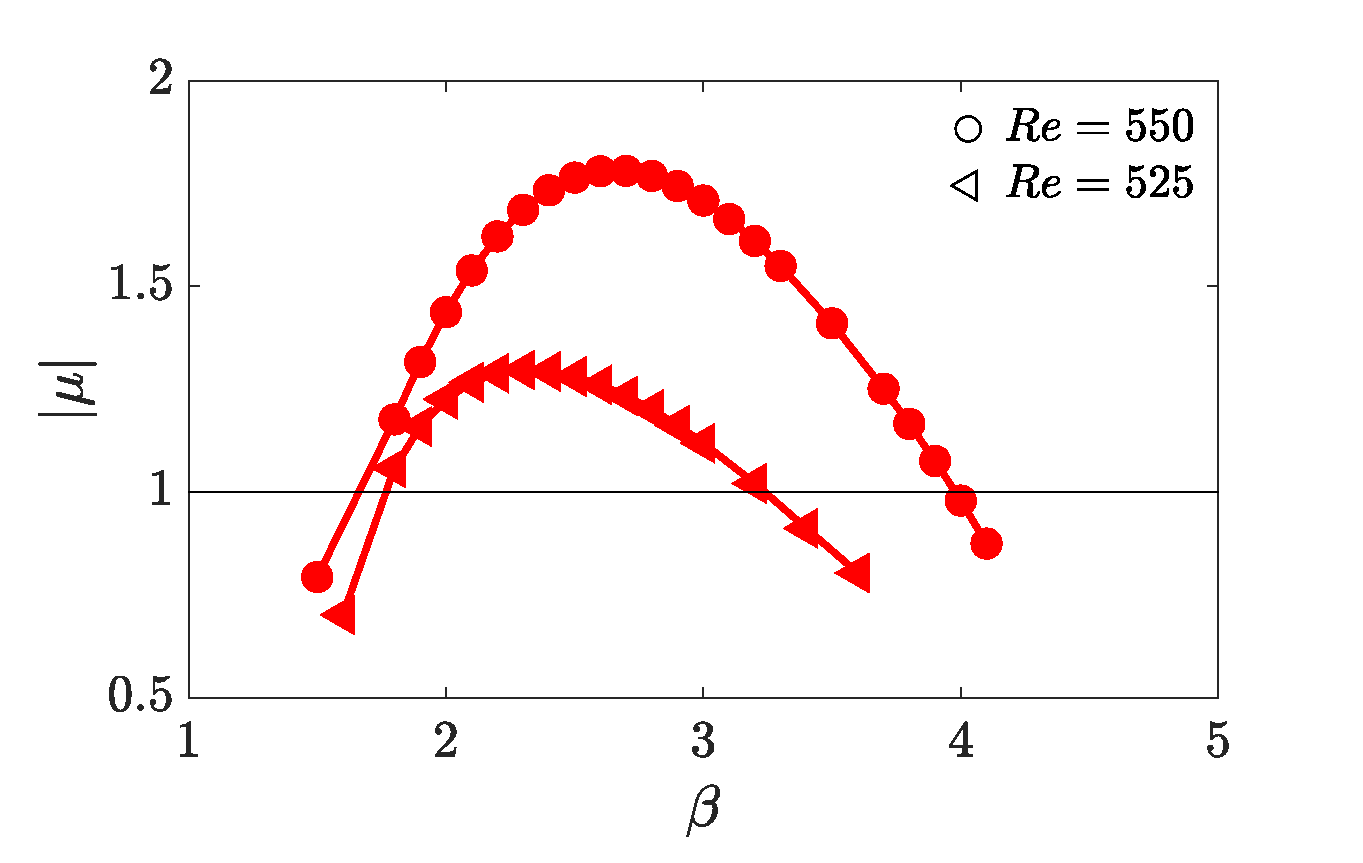
\includegraphics[width=0.49\textwidth]{./fig/AR5s/multipliers_AR5.eps}
  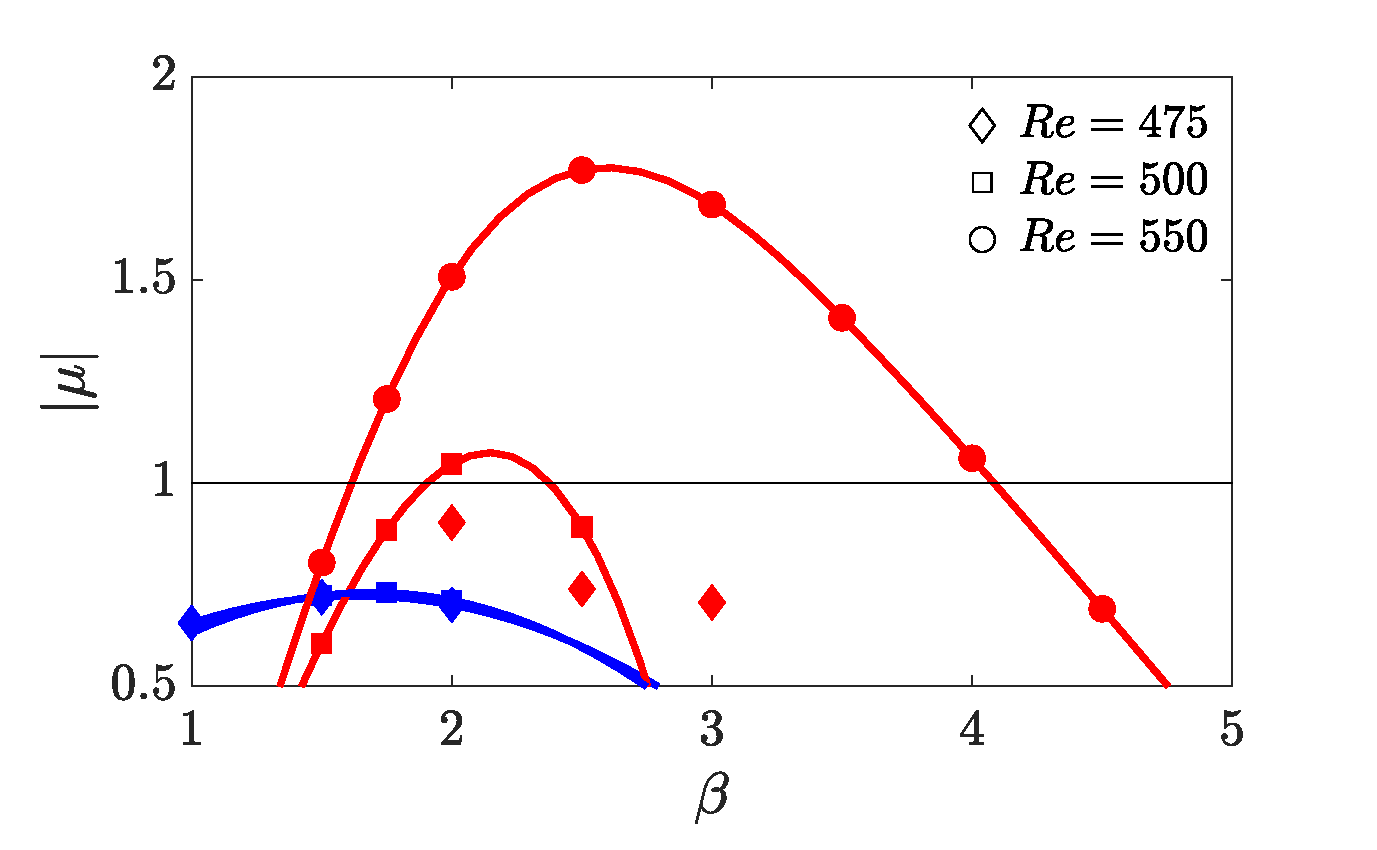
\includegraphics[width=0.49\textwidth]{./fig/AR5s/multipliers_AR5p25.eps}  
  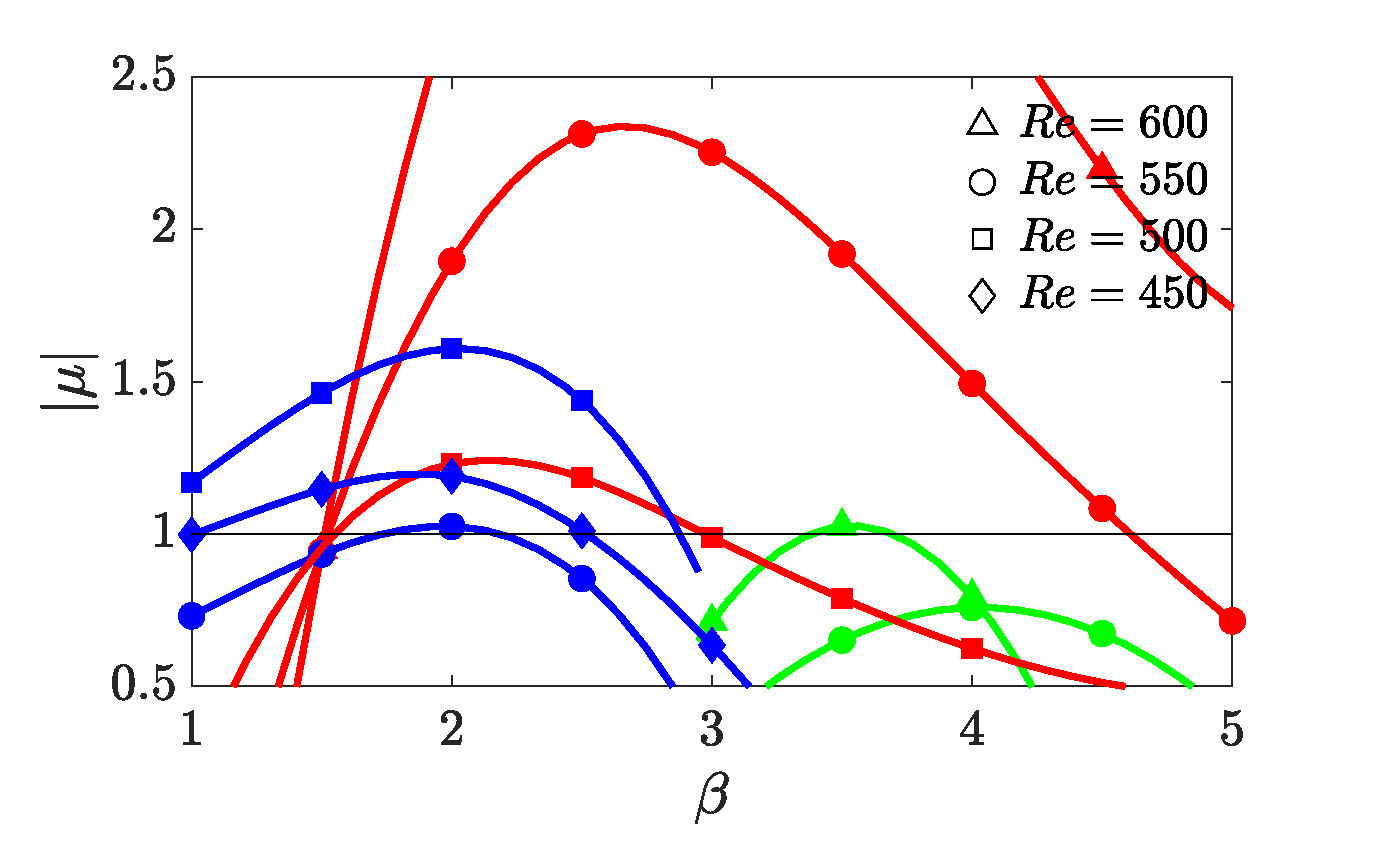
\includegraphics[width=0.49\textwidth]{./fig/AR5s/multipliers_AR5p5.eps}  
  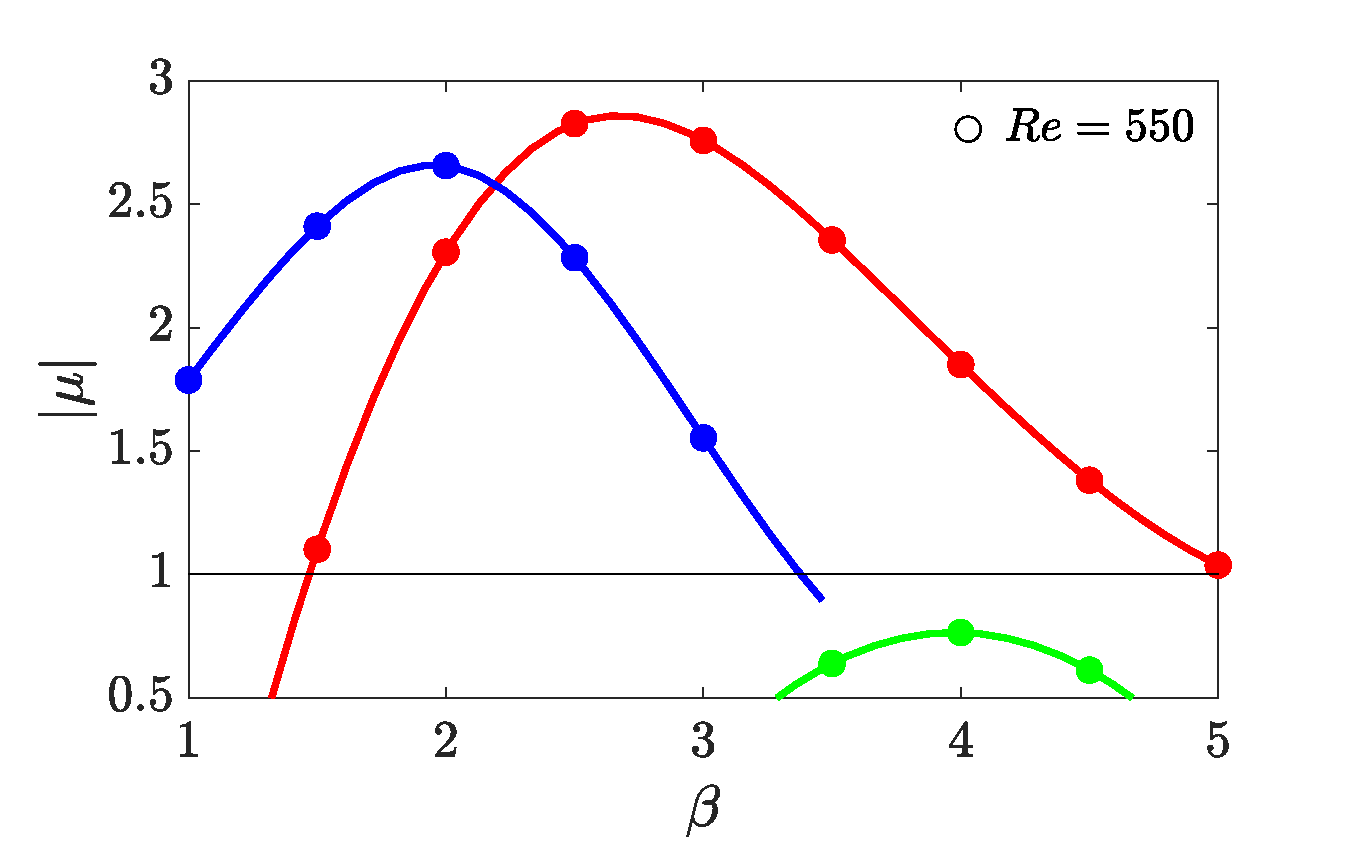
\includegraphics[width=0.49\textwidth]{./fig/AR5s/multipliers_AR5p75.eps}      
  \vspace{0.1cm}
  \begin{tikzpicture}
  \draw (-10,2) -- (8,2);
  \end{tikzpicture}
  \vspace{0.1cm}
  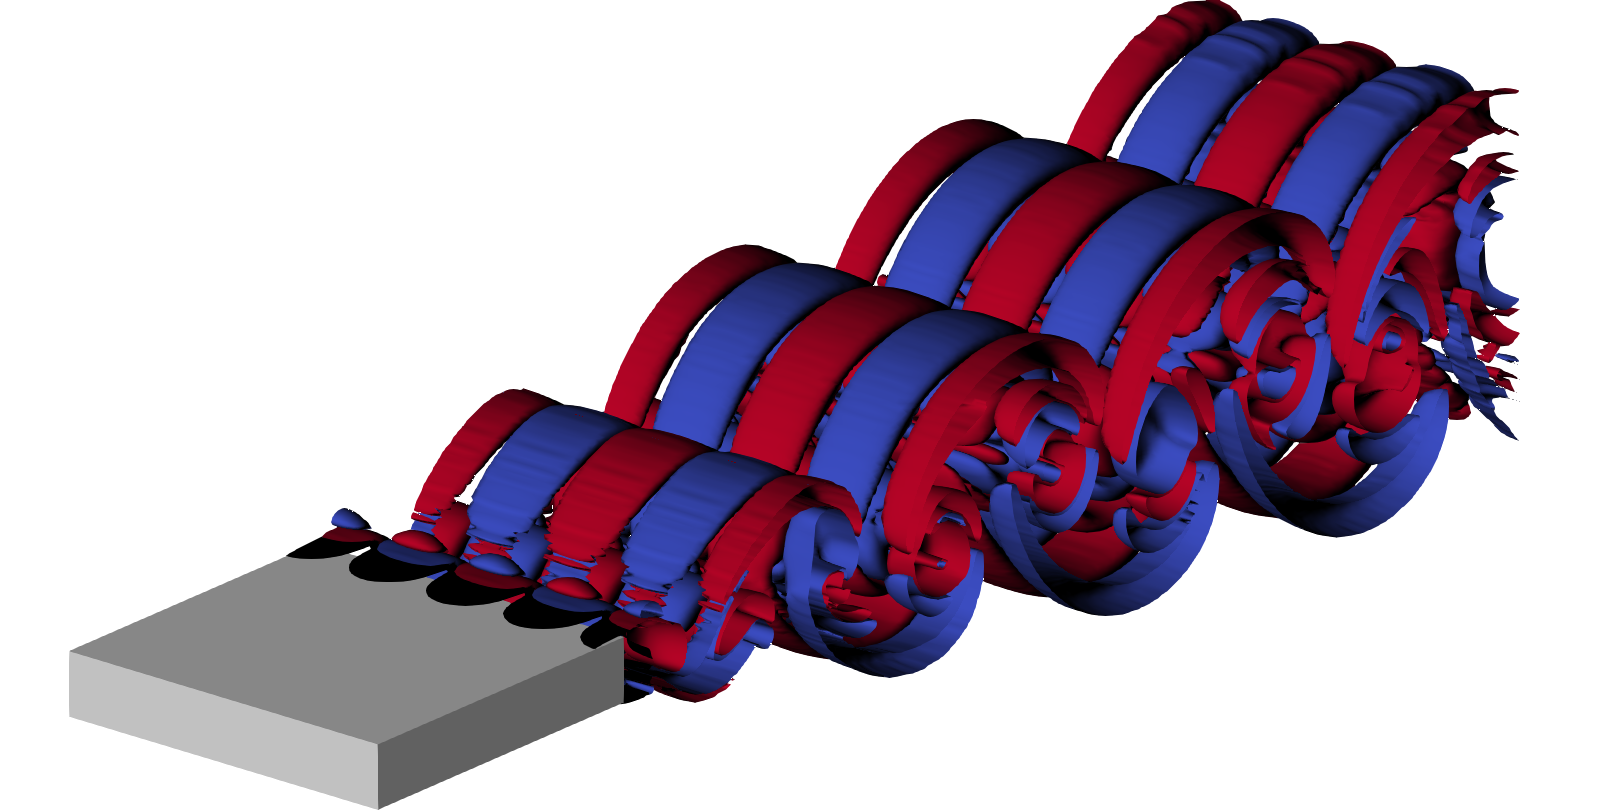
\includegraphics[width=0.32\textwidth]{./fig/AR5s/Floqetmode_beta_2_Re550_AR5p5_A.png}
  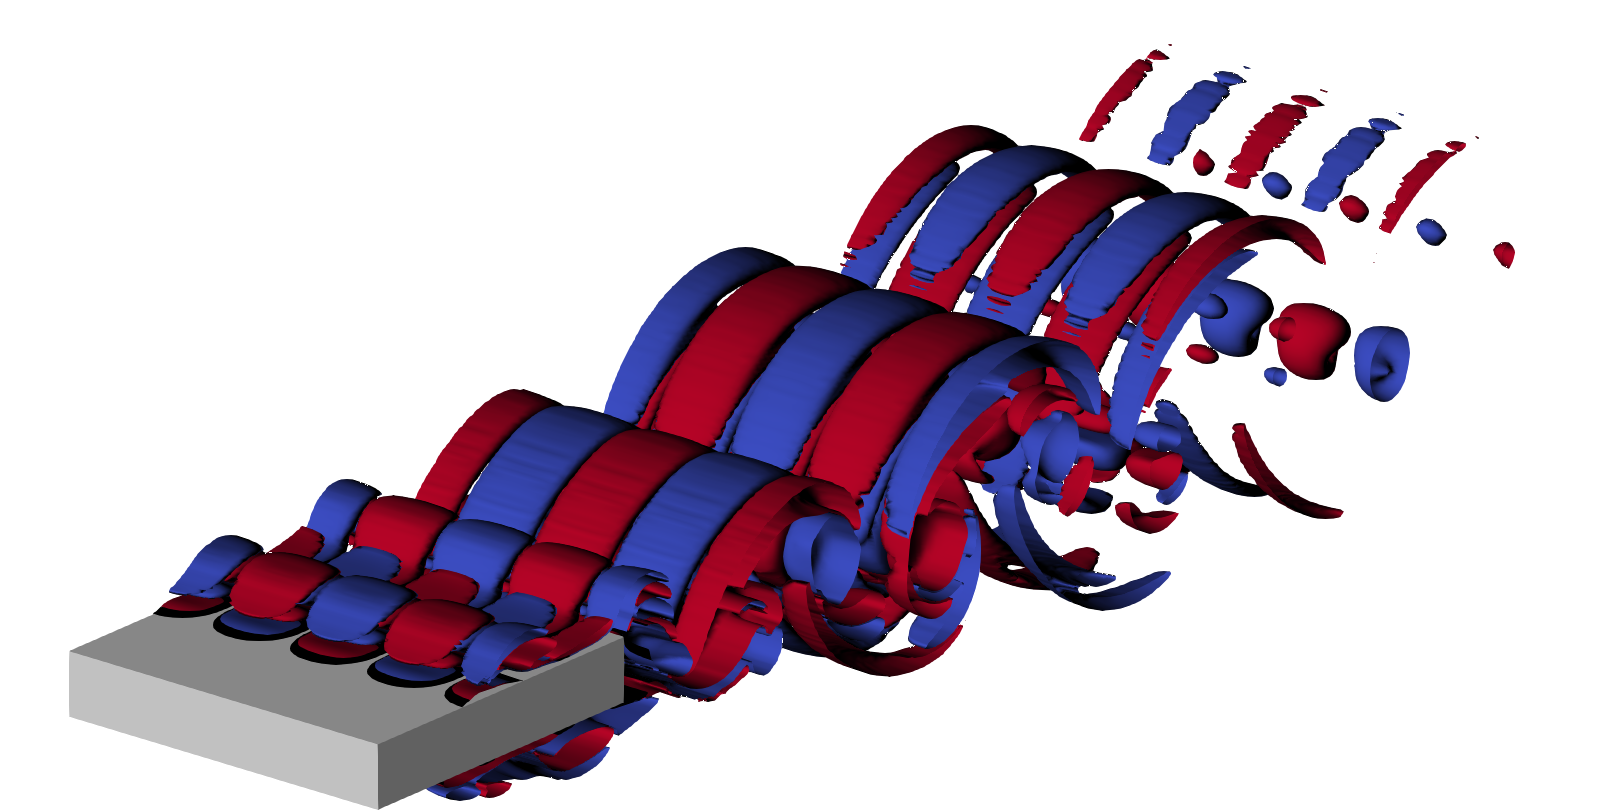
\includegraphics[width=0.32\textwidth]{./fig/AR5s/Floqetmode_beta_2_Re550_AR5p5_QS.png} 
  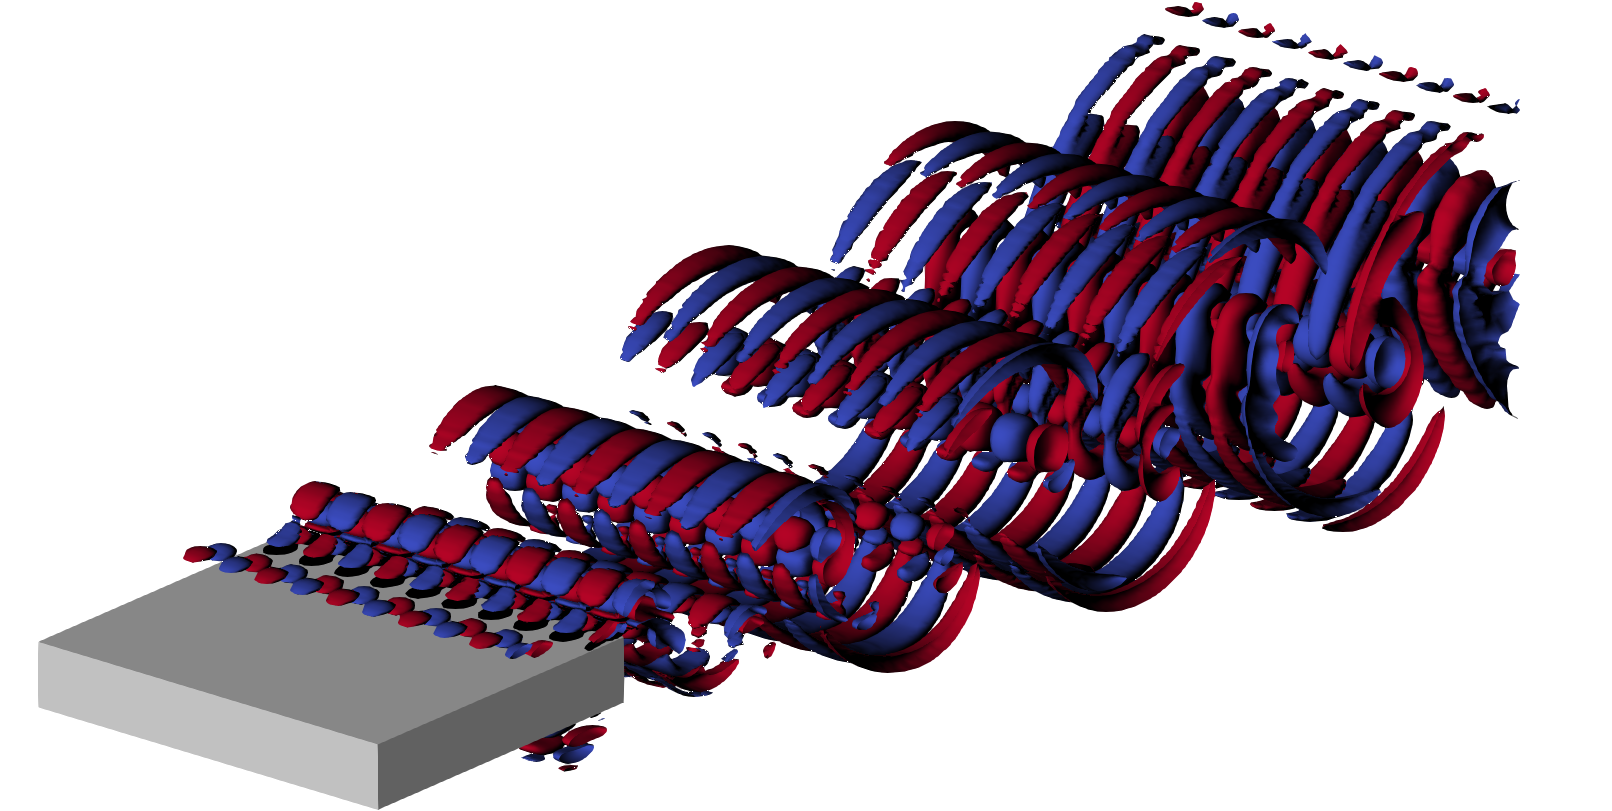
\includegraphics[width=0.32\textwidth]{./fig/AR5s/Floqetmode_beta_4p75_Re550_AR5p5_Ap.png}
  \vspace{0.1cm}
  \begin{tikzpicture}
  \draw (-10,2) -- (8,2);
  \end{tikzpicture}
  \vspace{0.1cm}
  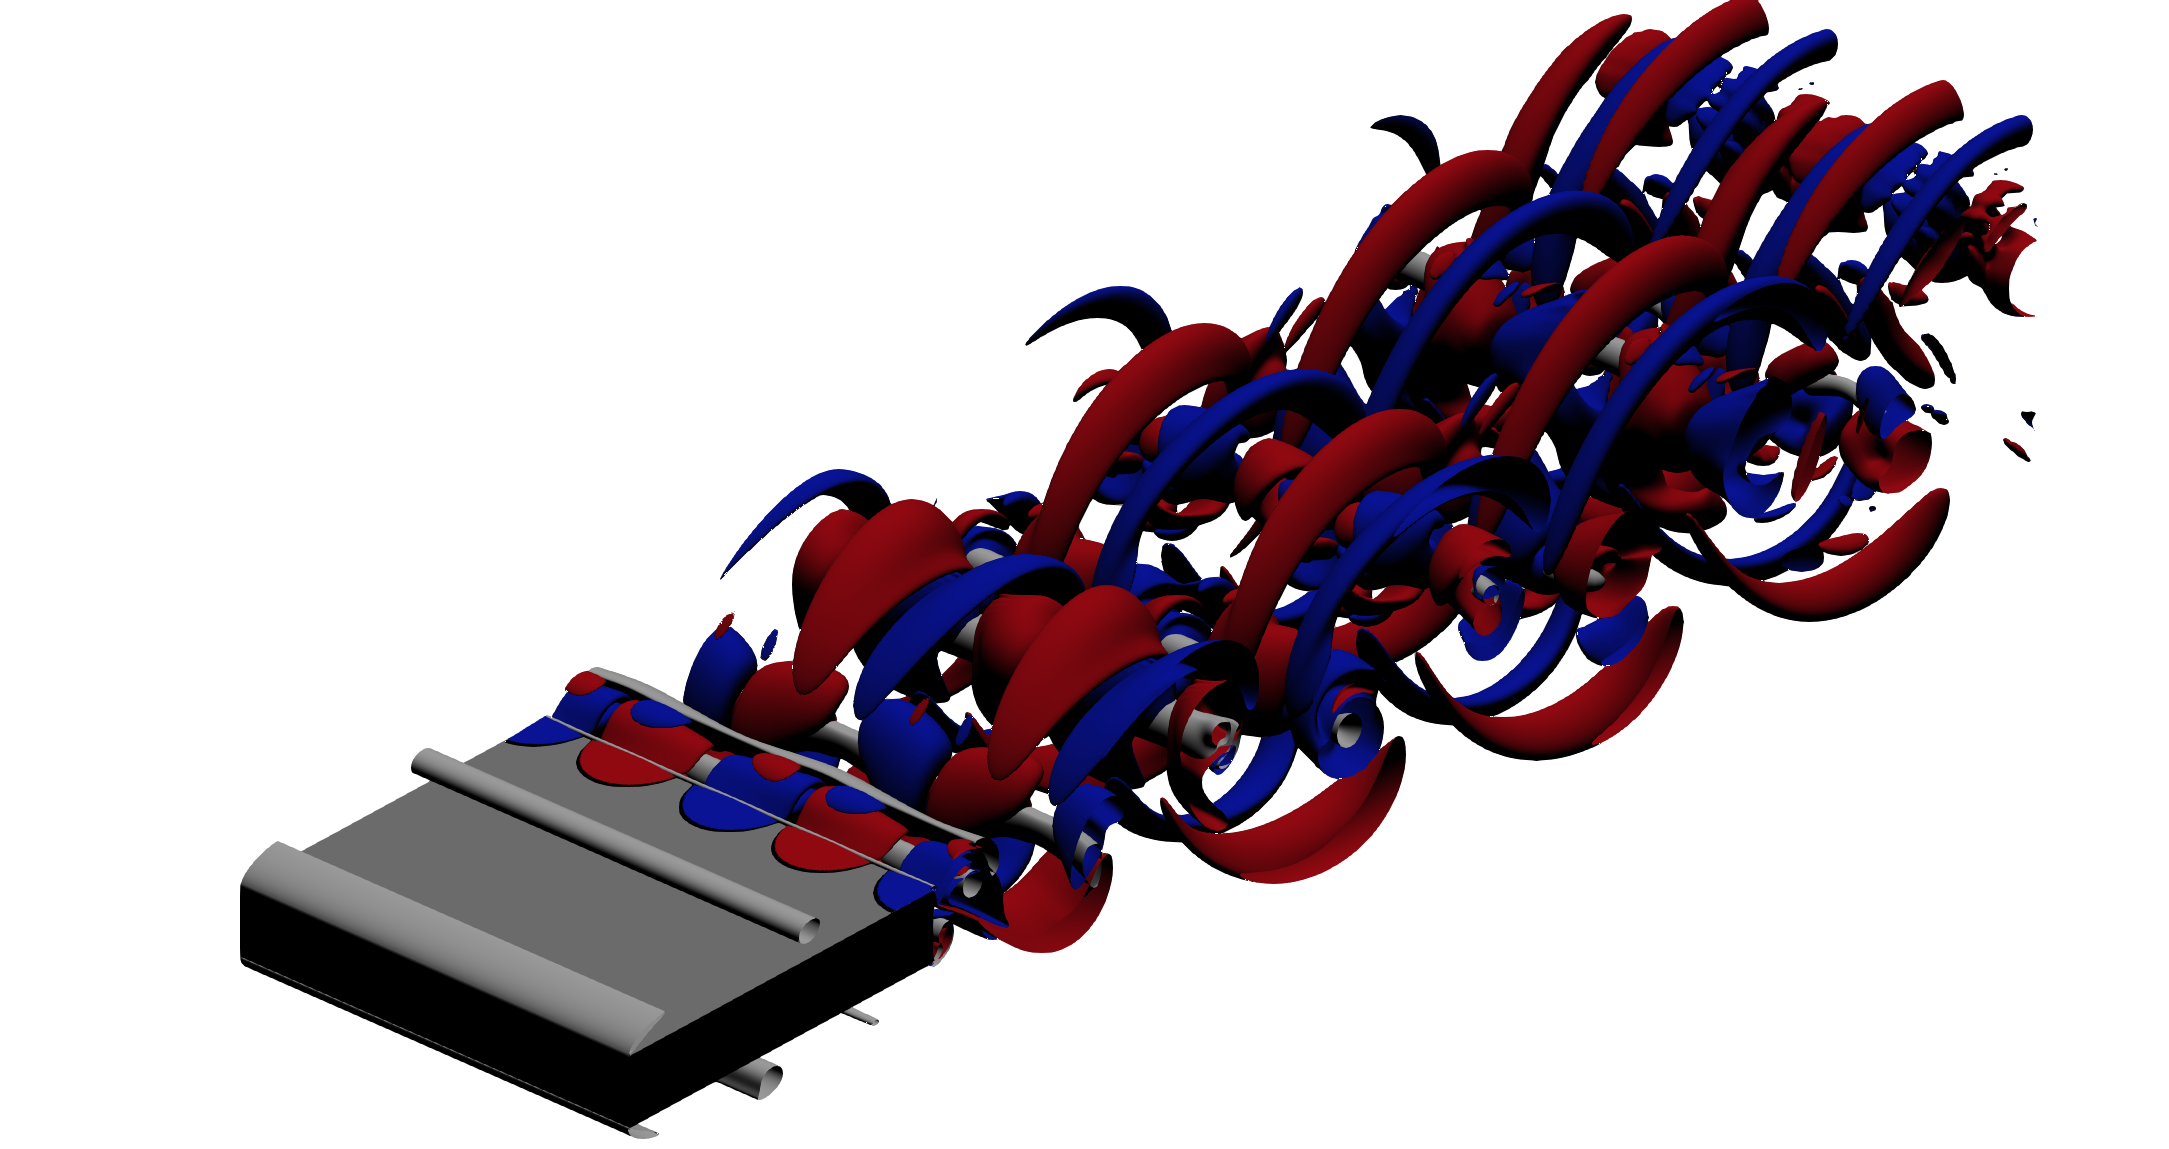
\includegraphics[width=0.49\textwidth]{./fig/AR5s/lambda2-AR55-Re450-3D.png}   
  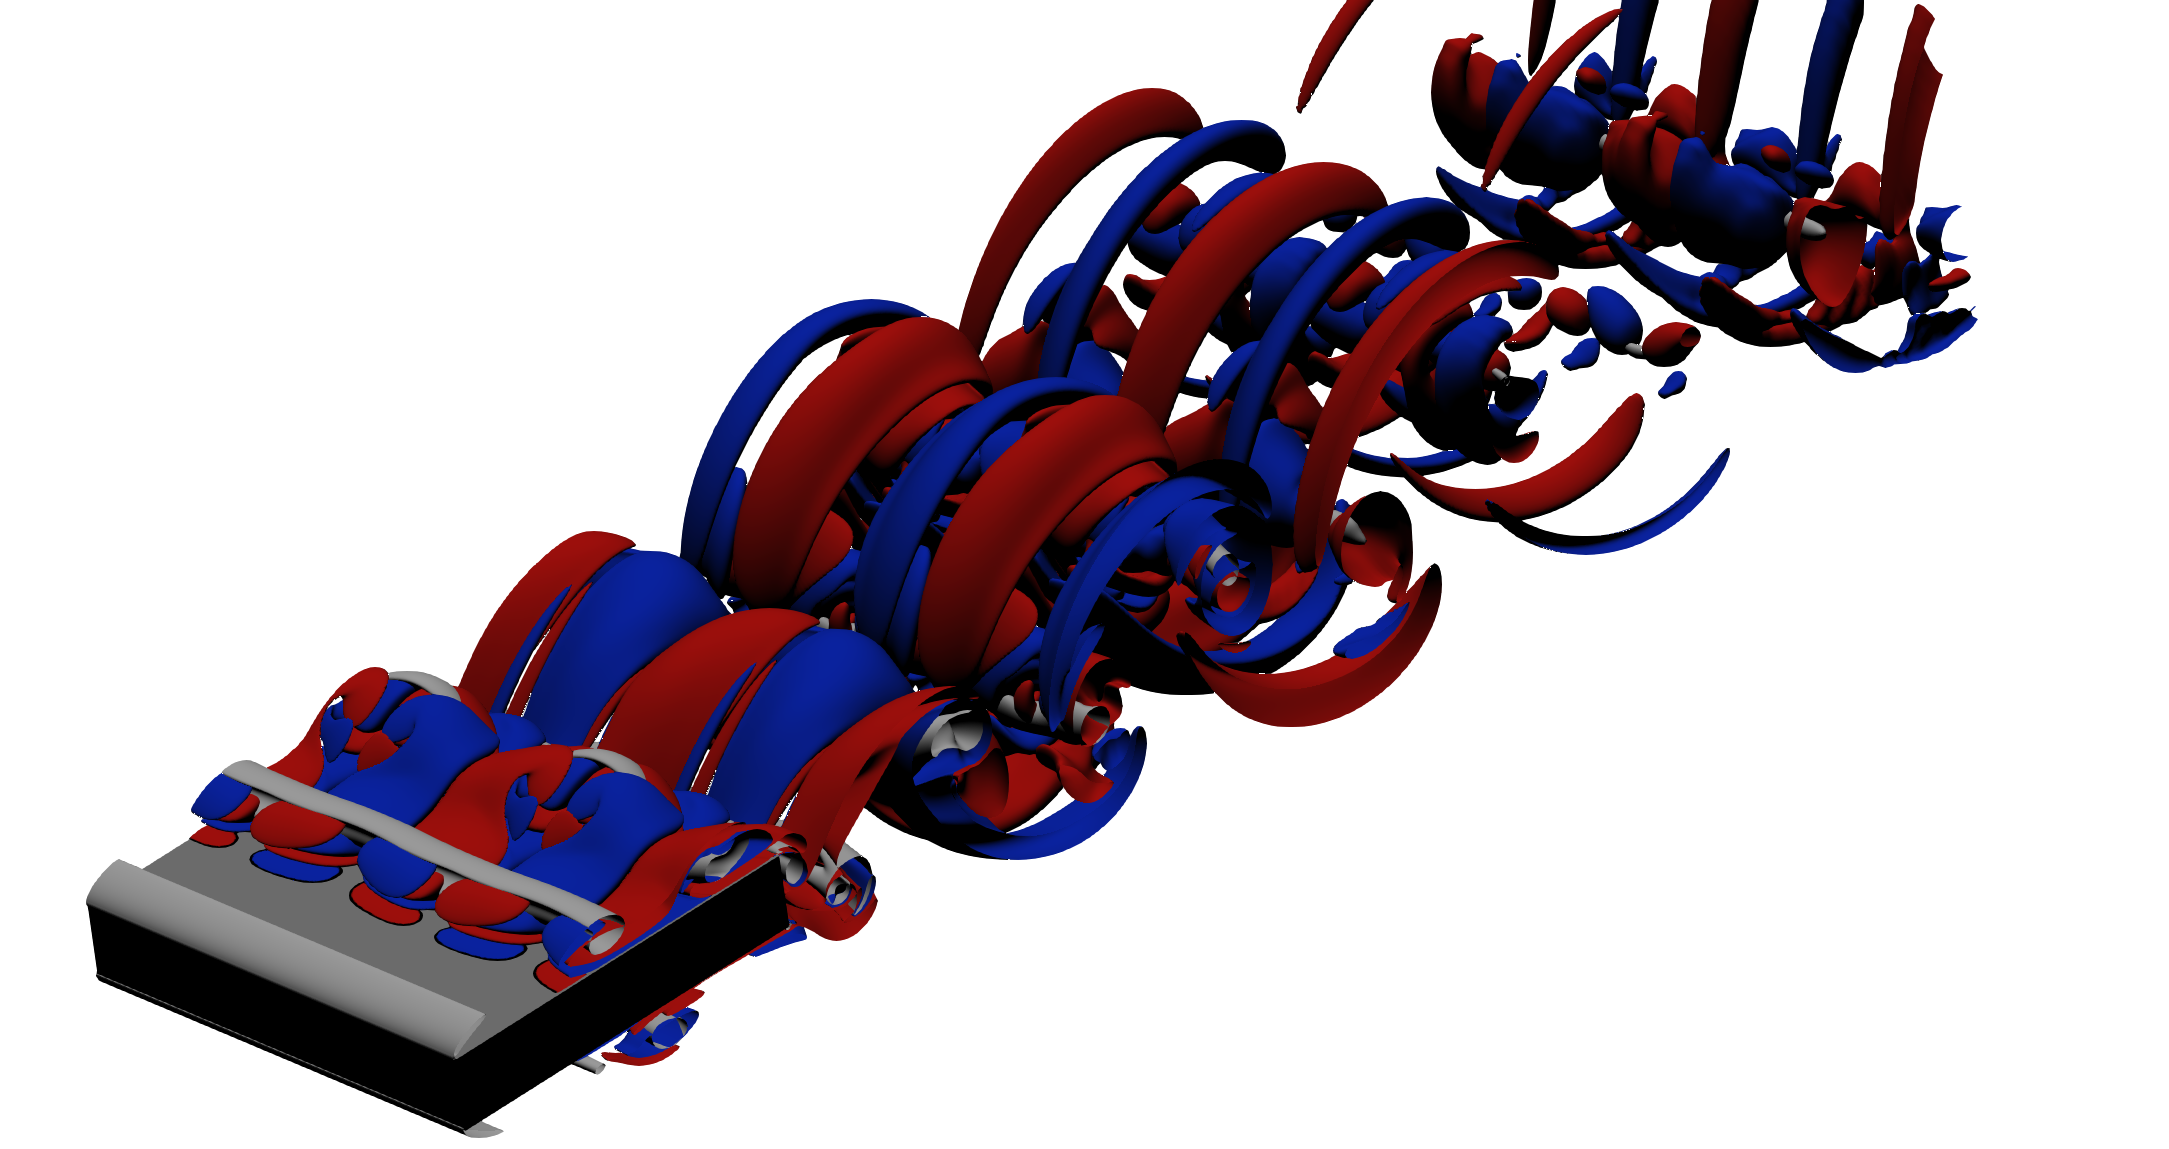
\includegraphics[width=0.49\textwidth]{./fig/AR5s/lambda2-AR55-Re500-3D.png}     
  \caption{Top: Floquet multipliers for $\AR=5$ (top left), $\AR=5.25$ (top right), $\AR=5.5$ (bottom left) and $\AR=5.75$ (bottom right). The red symbols refer to mode $QS$. The blue symbols refer to mode $A$. The green symbols refer to mode $B$. Different symbols refer to different $Re$. Centre: Floquet modes associated with mode A (left), mode QS (centre) and mode $A'$ for $\AR=5.5$ and $Re=550$. Bottom: Results from the 3D DNS for $\AR=5.5$. Left: $Re=450$, right: $Re=500$. It is thus clear that mode A dominates at smaller $Re$, while once mode $QS$ becomes unstable it dominates. Mode $A'$ has the same symmetries of mode $A$ and is a synchronous mode. The difference is that its characteristic wavelength is much smaller, with $\beta_c \approx 4.5$. XX CHECK MODE GREEN FOR $AR=5.5$ and $Re=600$. POTREBBE ESSERE CHE SONO DUE MODI SEPARATI? XX}
  \label{fig:mult_AR5s}
\end{figure} 

%\section{Bodies with $6 \le \AR \le 8$}

\begin{itemize}
  \item For these $\AR$, the secondary flow instability is due to mode $QS$ that leads to a three-dimensional state. Interestingly, for these $\AR$ mode $A$ is not detected. This is consistent with the fact that for this range of $\AR$, at the intermediate $Re$, the flow is driven by the LE vortex shedding, that modifies the flow dynamics in the near-wake region where the triggering mechanism of mode $A$ takes place. 
\end{itemize}

\begin{figure}
  \centering
  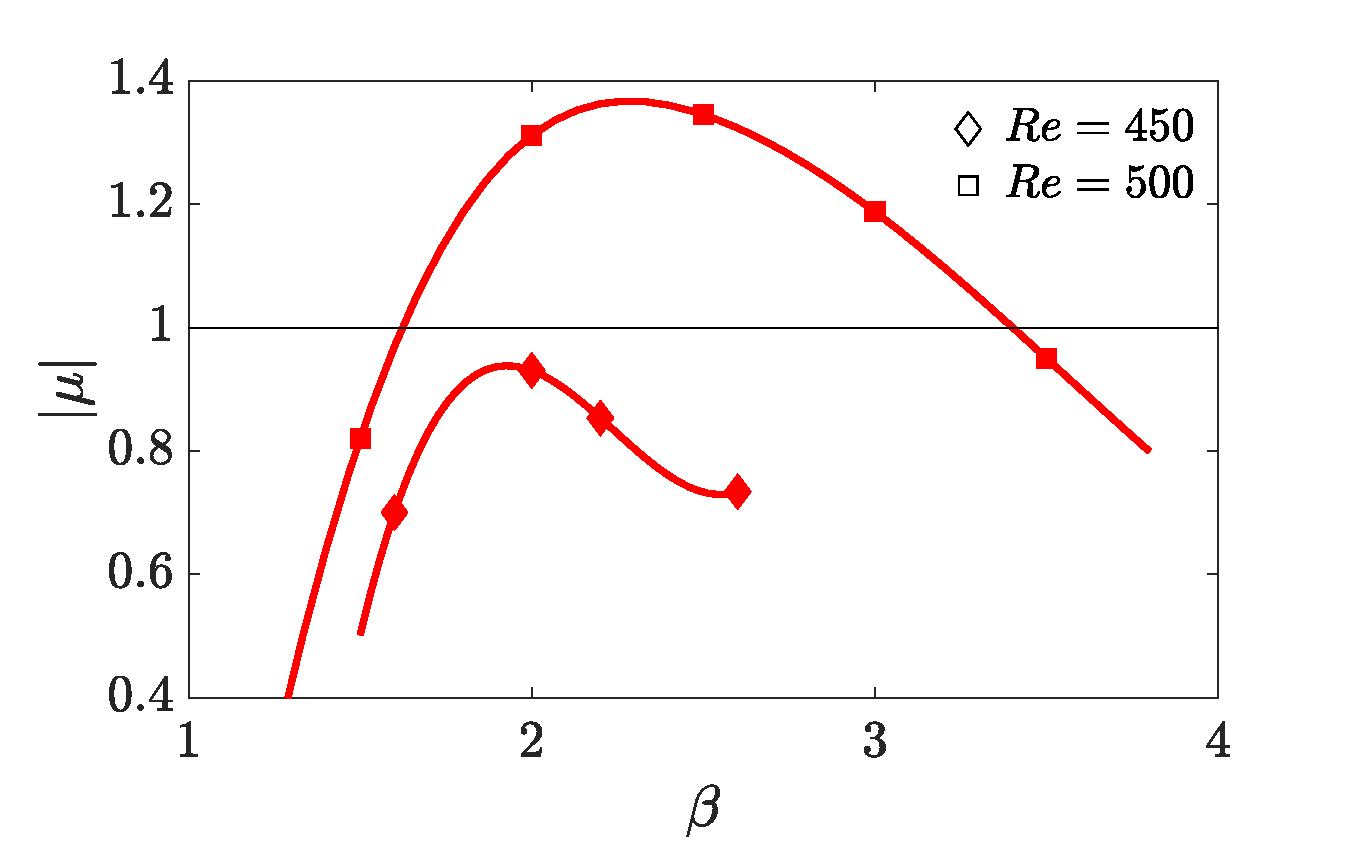
\includegraphics[width=0.49\textwidth]{./fig/AR7s/multipliers_AR6.eps}  
  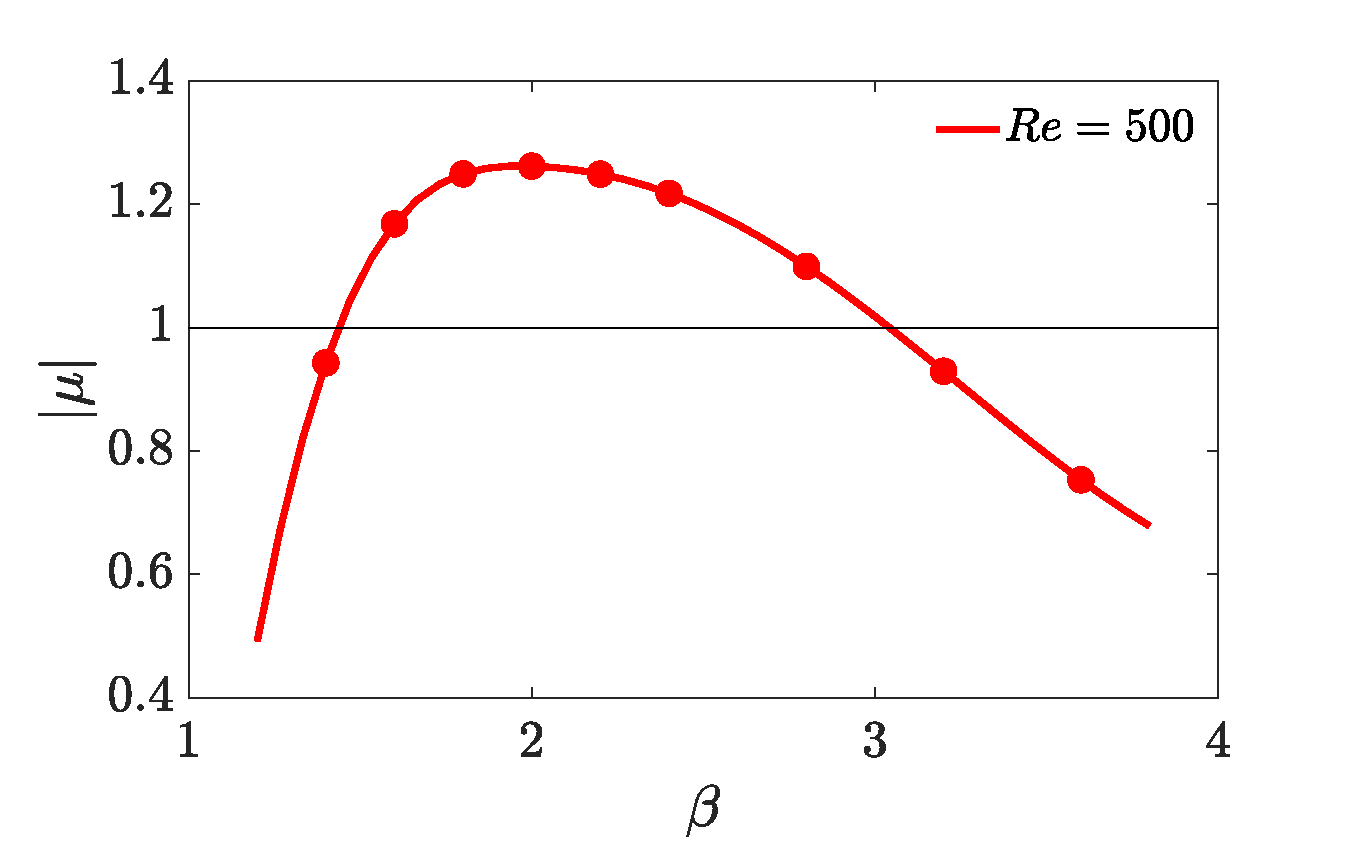
\includegraphics[width=0.49\textwidth]{./fig/AR7s/multipliers_AR7.eps}
  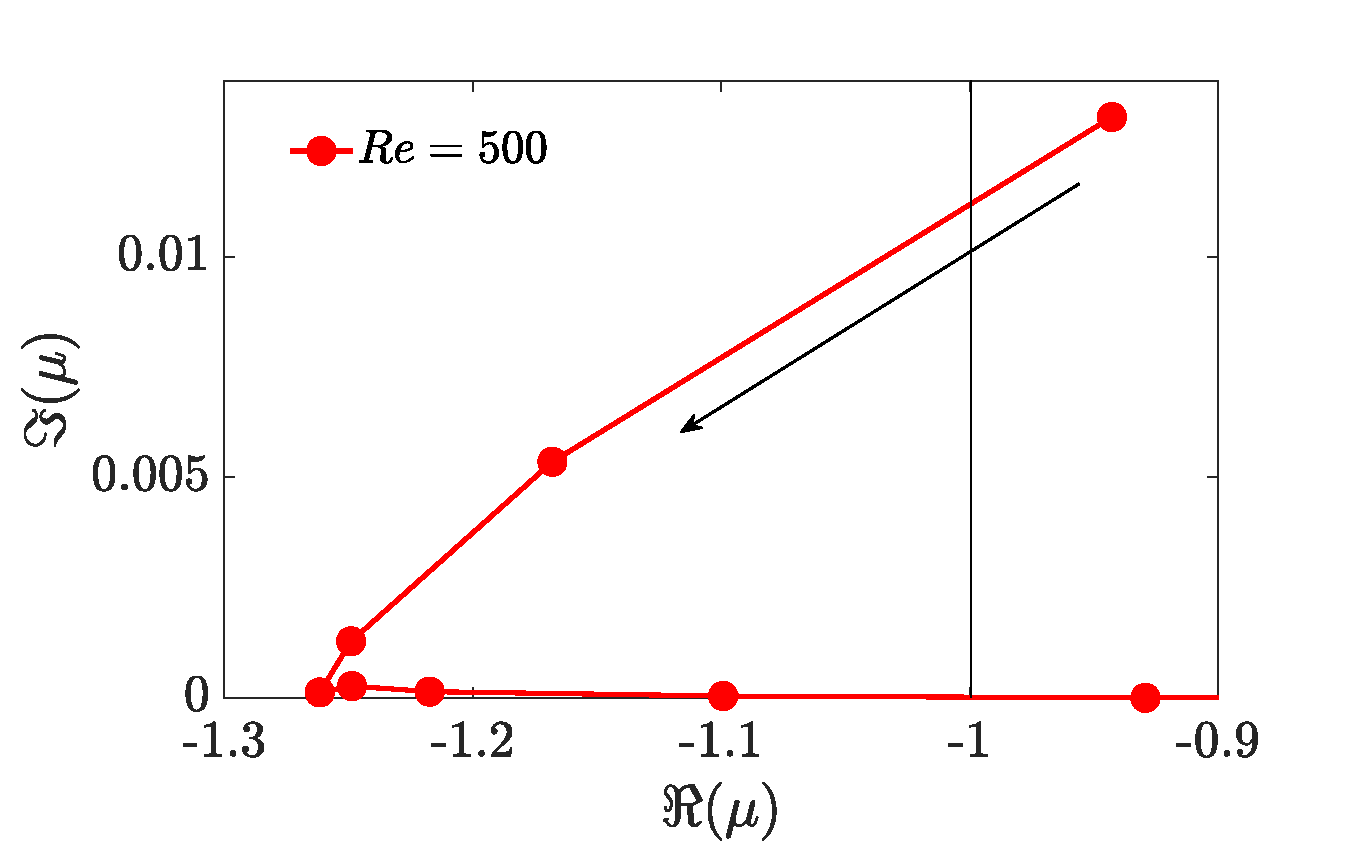
\includegraphics[width=0.49\textwidth]{./fig/AR7s/multipliers_AR7_b.eps}
  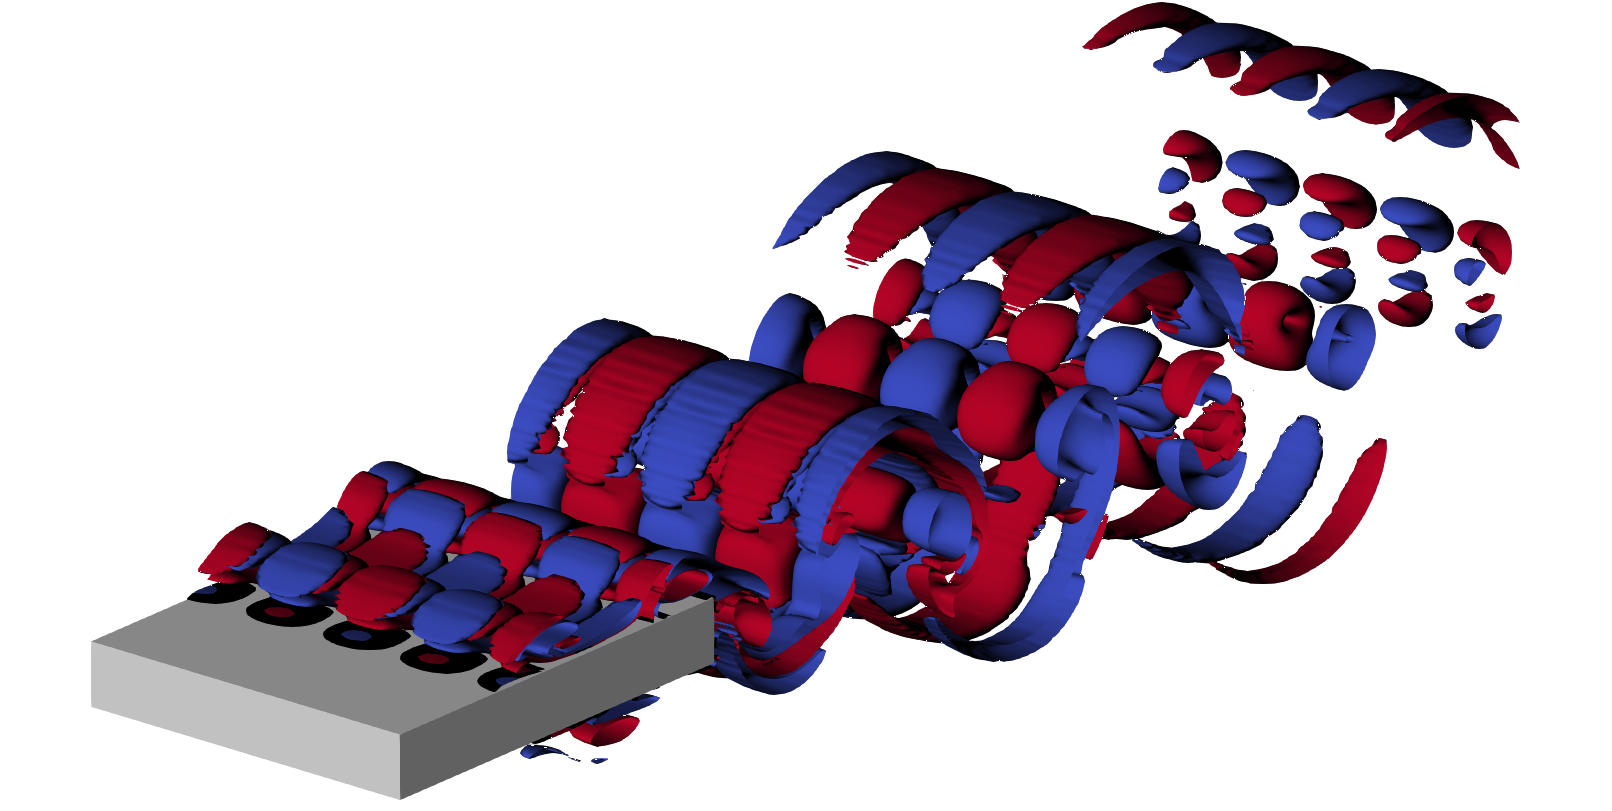
\includegraphics[width=0.7\textwidth]{./fig/AR7s/Floqetmode_beta_2p2_Re500_AR7.png}
  \caption{Floquet stability analysis for $\AR=6$ and $\AR=7$. Top: Floquet multipliers associated with the unstable branch. for $\AR=6$ (left) and $\AR=7$ (right). Centre: dependence of the real and imaginary parts of $\mu$ on $\beta$ for $\AR=7$. Bottom: three-dimensional reconstruction of the unstable Floquet mode for $\AR=7$. For these $\AR$s the secondary instability of the flow is due mode $QS$.}
  \label{fig:mult_AR7s}
\end{figure}

%\section{$\AR=9$}

\begin{figure}
  \centering
  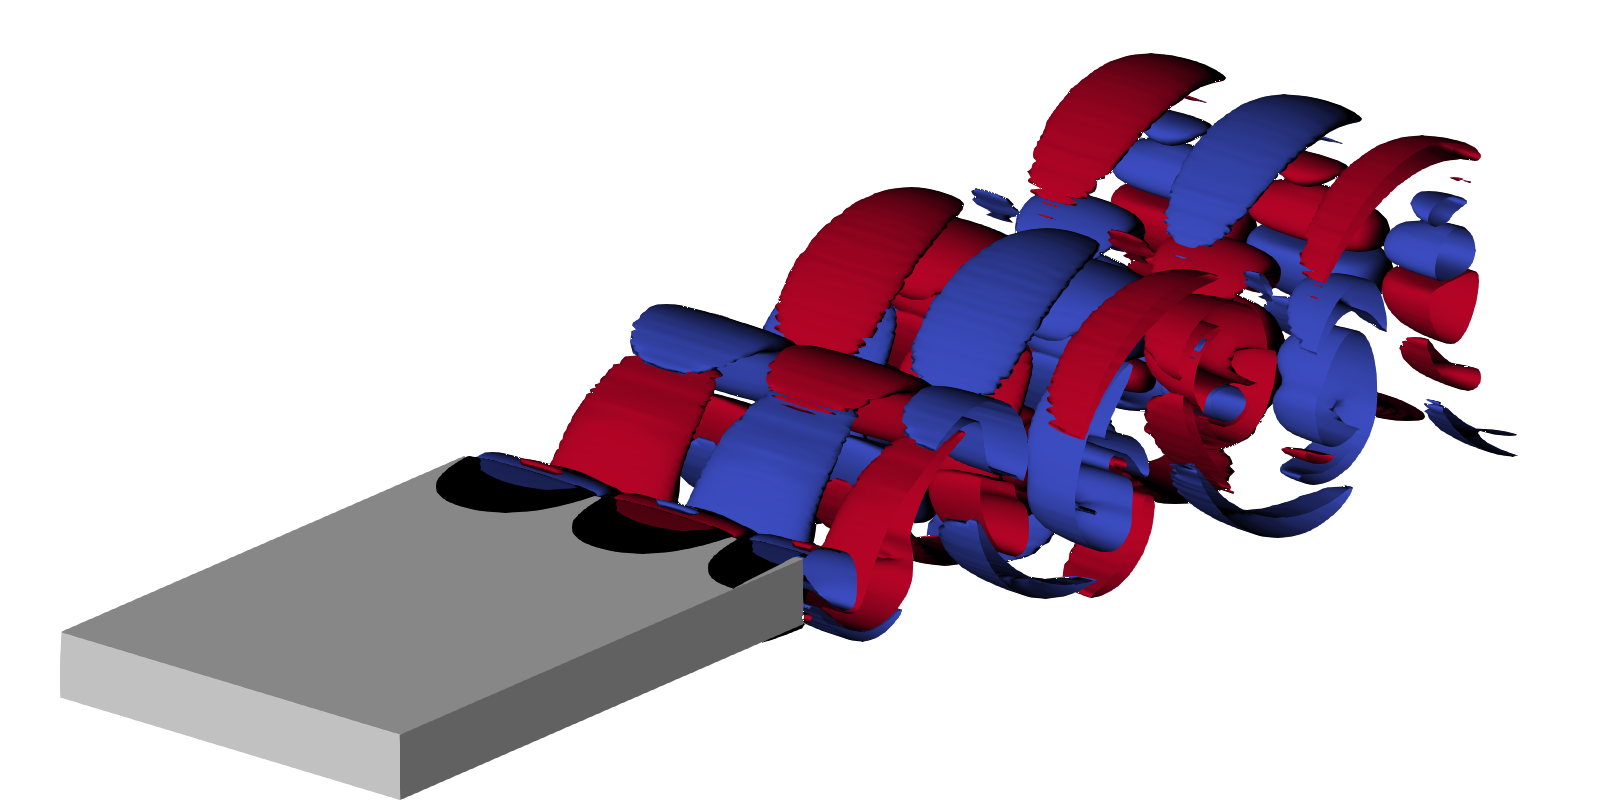
\includegraphics[width=0.49\textwidth]{./fig/AR9s/Floquet_AR9_Re400_beta1p2_modeA.png}  
  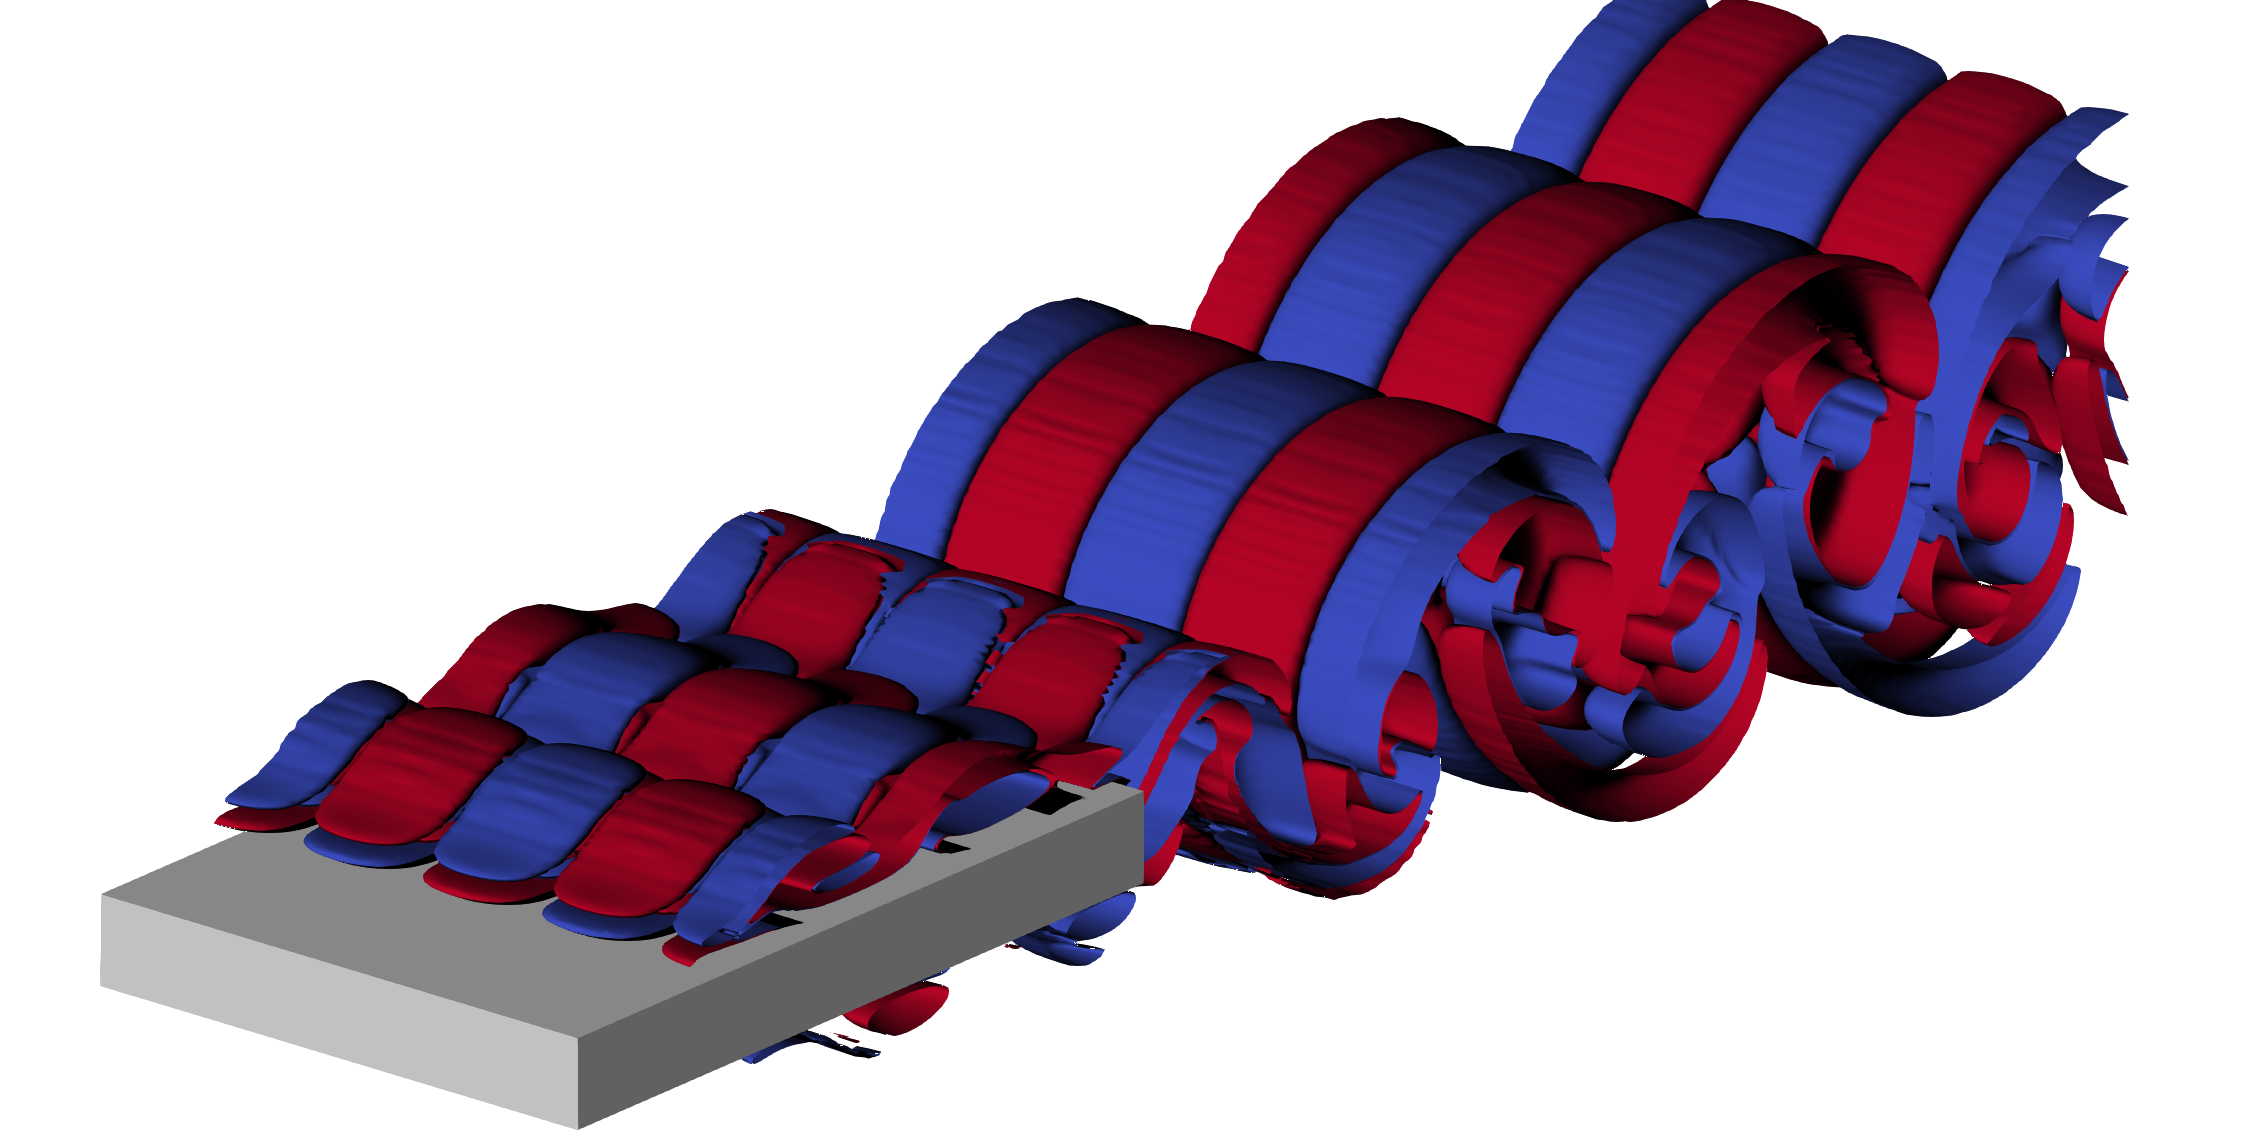
\includegraphics[width=0.49\textwidth]{./fig/AR9s/Floquet_AR9_Re450_beta2_modeQS.png}
  \caption{Reconstruction of the Floquet modes for $\AR=9$. Left: mode $A$, $Re=400$, $\beta=1.2$. Right: mode $QS$, $Re=450$, $\beta=2$.}
  \label{fig:mult_AR9s}
\end{figure}
